\documentclass[11pt]{article}

\usepackage[margin=1in]{geometry}
\usepackage{graphicx}
\usepackage{booktabs}
\usepackage{longtable}
\usepackage{enumitem}
\usepackage{xcolor}
\usepackage{hyperref}
\usepackage{listings}
\usepackage{caption}
\usepackage{amsmath}
\usepackage{tikz}
\usetikzlibrary{arrows.meta,positioning,shapes.geometric}

\hypersetup{
  colorlinks=true,
  linkcolor=blue,
  urlcolor=blue,
  citecolor=blue
}

\title{\textbf{Tennis/Pickleball Single-Camera Tracking System}\\[4pt]
Progress Report \& Task Allocation}
\author{
  \textbf{Course:} Computer Vision \\
  \textbf{Instructor:} Nguyen Duc Dung \\[6pt]
  \textbf{Team Members:} \\
  1.~Pham Hoang An \quad
  2.~Dao Duy Anh \quad
  3.~Duong Vu Duc \\
  4.~Nguyen Duc Dat \quad
  5.~Bui Dinh Nguyen Minh \\[6pt]
  \textbf{GitHub:} \url{https://github.com/AnHgPham/cv}
}
\date{\textbf{Report date:} February 23, 2026}

\lstset{
  basicstyle=\ttfamily\small,
  breaklines=true,
  frame=single,
  numbers=left,
  numberstyle=\tiny,
  keywordstyle=\color{blue},
  commentstyle=\color{gray},
  stringstyle=\color{teal}
}

\begin{document}
\maketitle
\tableofcontents
\newpage

% ============================================================================
\section{Abstract}
This project implements a complete single-camera computer vision pipeline for
tennis and pickleball video analysis.  The system processes monocular video
(25--30\,fps) and produces:
\begin{itemize}[nosep]
  \item Real-time ball trajectory detection and tracking,
  \item Player detection with persistent identity assignment,
  \item Court-line detection and image-to-court homography estimation,
  \item Physics-based 3D trajectory reconstruction of the ball,
  \item Bounce detection with in/out classification,
  \item Annotated output video with bird's-eye mini-map and heatmaps.
\end{itemize}
This report presents the current implementation status, documents bugs
identified and fixed during development, highlights remaining issues
(primarily an incorrect homography due to multi-court interference), and
defines a task allocation for a 5-member team to deliver a stable, evaluated
system.

% ============================================================================
\section{Repository and Project Structure}
\label{sec:repo}

The full source code is hosted on GitHub:
\begin{itemize}[nosep]
  \item Repository: \url{https://github.com/AnHgPham/cv}
  \item Project root: \texttt{cv/tennis-pickleball-tracker/}
\end{itemize}

\subsection{Directory Layout}
\begin{lstlisting}[basicstyle=\ttfamily\footnotesize,numbers=none]
tennis-pickleball-tracker/
|-- src/
|   |-- court_detection.py      # Module 1 (~25 KB, ~720 lines)
|   |-- object_detection.py     # Module 2 (~35 KB, ~400 lines)
|   |-- object_tracking.py      # Module 3 (~24 KB, ~540 lines)
|   |-- trajectory_3d.py        # Module 4a (~31 KB, ~680 lines)
|   |-- in_out_classifier.py    # Module 4b (~9 KB, ~250 lines)
|   |-- pipeline.py             # Module 5a (~36 KB, ~940 lines)
|   |-- visualization.py        # Module 5b (~21 KB, ~630 lines)
|   `-- __init__.py
|-- notebooks/
|   |-- 01_data_exploration.ipynb
|   |-- 02_court_detection.ipynb
|   |-- 03_ball_detection.ipynb
|   |-- 04_tracking.ipynb
|   `-- 05_3d_reconstruction.ipynb
|-- configs/court_config.yaml
|-- data/raw/                   # Input videos (not in git)
|-- outputs/                    # Generated results (not in git)
|-- run_pipeline.py             # CLI entry point
|-- test_fix.py                 # Single-frame debug script
`-- report.tex                  # This report
\end{lstlisting}

% ============================================================================
\section{System Architecture}
\label{sec:arch}

\subsection{Pipeline Flow Diagram}

\begin{center}
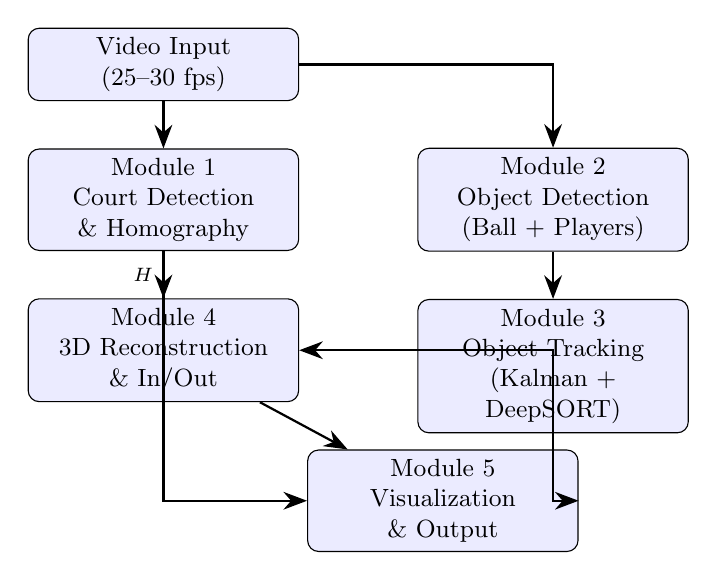
\begin{tikzpicture}[
  node distance=0.6cm and 1.5cm,
  block/.style={rectangle, draw, fill=blue!8, text width=3.2cm,
    align=center, rounded corners, minimum height=0.9cm, font=\small},
  arrow/.style={-{Stealth[length=3mm]}, thick}
]
  \node[block] (input) {Video Input\\(25--30 fps)};
  \node[block, below=of input] (court) {Module 1\\Court Detection\\\& Homography};
  \node[block, right=of court] (detect) {Module 2\\Object Detection\\(Ball + Players)};
  \node[block, below=of detect] (track) {Module 3\\Object Tracking\\(Kalman + DeepSORT)};
  \node[block, below=of court] (traj) {Module 4\\3D Reconstruction\\\& In/Out};
  \node[block, below right=0.6cm and 0.1cm of traj] (viz) {Module 5\\Visualization\\\& Output};

  \draw[arrow] (input) -- (court);
  \draw[arrow] (input.east) -| (detect);
  \draw[arrow] (court) -- node[left, font=\scriptsize]{$H$} (traj);
  \draw[arrow] (detect) -- (track);
  \draw[arrow] (track.south) |- (traj.east);
  \draw[arrow] (traj) -- (viz);
  \draw[arrow] (track.south) |- (viz.east);
  \draw[arrow] (court.south) |- (viz.west);
\end{tikzpicture}
\end{center}

\subsection{Per-Frame Processing Steps}
For every frame $t$ in the input video:
\begin{enumerate}[nosep]
  \item \textbf{Court Detection (Module 1):}
        Detect white court lines via HSV thresholding, extract edges with
        Canny, find line segments with Hough transform, compute line
        intersections, select 4 court corners, and estimate a $3\times3$
        homography matrix $H$ that maps pixel coordinates $(u,v)$ to
        real-world court coordinates $(x_c, y_c)$ in metres.
  \item \textbf{Object Detection (Module 2):}
        Run YOLOv8 on the frame to detect persons and sports balls.
        Supplement with a classical contour-based ball detector for small
        tennis balls that YOLO may miss.  Apply non-maximum suppression
        (NMS) to remove duplicate detections.
  \item \textbf{Player Filtering (Module 5):}
        Score each player detection by (a)~x-distance from frame centre
        (weight 0.60), (b)~perspective-consistent size (weight 0.25),
        (c)~YOLO confidence (weight 0.15).  Hard-reject detections whose
        centre exceeds 40\% of frame width from the frame centre.  Keep
        top $k$ (default $k=4$ for doubles).
  \item \textbf{Tracking (Module 3):}
        Update the ball Kalman filter with the new detection (or predict
        if no detection).  Use Lucas-Kanade optical flow as a secondary
        motion estimate.  Update the player tracker (DeepSORT or IoU
        fallback) to maintain persistent IDs.
  \item \textbf{3D Reconstruction (Module 4):}
        Project the tracked ball position through $H$ to obtain court
        coordinates.  Estimate ball height using a physics model
        (gravity $g = 9.81$\,m/s$^2$, air drag).  Detect bounces from
        trajectory direction changes.  Classify each bounce as in or out
        by checking whether $(x_c, y_c)$ falls within the standard court
        rectangle.
  \item \textbf{Visualization (Module 5):}
        Draw bounding boxes, ball trajectory trail, info overlay, and
        compose the output frame with a side-panel mini-map and frame
        metadata.
\end{enumerate}

% ============================================================================
\section{Module Details}
\label{sec:modules}

\subsection{Module 1: Court Detection \& Homography}
\textbf{File:} \texttt{src/court\_detection.py} \\
\textbf{Owner:} Pham Hoang An

\subsubsection{Technical Approach}
\begin{enumerate}[nosep]
  \item \textbf{Pre-processing:} Convert BGR $\rightarrow$ HSV; threshold
        for white pixels (H: 0--180, S: 0--50, V: 180--255); morphological
        dilation (2 iterations) and erosion (1 iteration) with a
        $5\times5$ rectangular kernel.
  \item \textbf{Edge Detection:} Canny with thresholds (50, 150).
  \item \textbf{Line Detection:} Probabilistic Hough Transform
        ($\rho=1$, $\theta=\pi/180$, threshold$=100$,
        minLineLength$=50$, maxLineGap$=30$).
  \item \textbf{Line Classification:} Separate into horizontal and
        vertical groups based on angle ($\pm30^\circ$ from horizontal/
        vertical).  Merge similar lines within 30\,px distance.
  \item \textbf{Intersection Computation:} Compute all pairwise
        intersections of horizontal and vertical lines.
  \item \textbf{Corner Selection:} Compute centroid of all intersection
        points; assign each point to a quadrant (TL, TR, BL, BR)
        relative to the centroid; pick one representative per quadrant.
  \item \textbf{Homography:} Compute $H$ via \texttt{cv2.findHomography}
        with RANSAC (reproj.\ threshold $=5.0$\,px) mapping 4 image
        corners $\rightarrow$ standard court corners
        (tennis: $23.77 \times 10.97$\,m).
\end{enumerate}

\subsubsection{Additional Components}
\begin{itemize}[nosep]
  \item \textbf{SIFT Court Matcher:} Computes frame-to-frame homography
        using SIFT keypoints + FLANN matcher + Lowe's ratio test, enabling
        camera-motion compensation.
  \item \textbf{Deep Court Detector (scaffolded):} CNN-based keypoint
        regression using a ResNet-18 backbone.  Not yet trained.
\end{itemize}

\subsubsection{Known Constants}
Standard tennis court keypoints are defined in \texttt{TENNIS\_COURT\_KEYPOINTS}
(21 points in metres) and \texttt{TENNIS\_COURT\_CORNERS} (4 corners).
Pickleball court keypoints are also defined.

\subsubsection{Applied Knowledge}
Image processing (colour spaces, morphology), Canny edge detection, Hough
transform, SIFT feature matching, homography estimation (DLT + RANSAC),
convolutional neural networks.

% --------------------------------------------------------------------------
\subsection{Module 2: Object Detection}
\textbf{File:} \texttt{src/object\_detection.py} \\
\textbf{Owner:} Dao Duy Anh

\subsubsection{Detectors Implemented}
\begin{enumerate}[nosep]
  \item \textbf{YOLODetector:} Wraps Ultralytics YOLOv8.
    \begin{itemize}[nosep]
      \item Supports both COCO-pretrained models (class 0 = person, class
            32 = sports ball) and custom-trained models (user-defined
            class map).
      \item Configurable confidence threshold (default 0.25), device
            (CPU/CUDA).
      \item Detected 9 persons in a typical frame of our test video.
    \end{itemize}
  \item \textbf{ClassicalBallDetector:} A multi-stage pipeline for
        detecting small tennis balls that YOLO often misses:
    \begin{itemize}[nosep]
      \item HSV colour filtering for yellow/green tennis balls
            (H: 20--50, S: 50--255, V: 120--255).
      \item Contour extraction with circularity filter
            ($4\pi A / P^2 > 0.6$).
      \item Size filtering (radius 3--30\,px).
      \item Motion detection via frame differencing.
      \item Court-region filtering (optional, uses court polygon).
    \end{itemize}
  \item \textbf{TrackNetDetector (scaffolded):} A specialised heatmap
        regression network that uses 3 consecutive frames as input to
        detect fast-moving balls.
  \item \textbf{ClassicalPlayerDetector:} HOG + SVM or Haar cascade
        baseline for player detection.
  \item \textbf{FasterRCNNDetector (scaffolded):} Two-stage detector
        using torchvision's pre-trained Faster R-CNN.
\end{enumerate}

\subsubsection{Detection Priority}
The pipeline tries detectors in this order: classical $\rightarrow$ YOLO
$\rightarrow$ TrackNet.  The first detector to return a ball detection
``wins'' for that frame.

\subsubsection{Applied Knowledge}
Feature engineering (HOG, Haar), deep object detection (YOLO, Faster R-CNN),
heatmap regression (TrackNet), non-maximum suppression, colour space
analysis, contour geometry.

% --------------------------------------------------------------------------
\subsection{Module 3: Object Tracking}
\textbf{File:} \texttt{src/object\_tracking.py} \\
\textbf{Owner:} Duong Vu Duc

\subsubsection{Ball Tracking}
\begin{itemize}[nosep]
  \item \textbf{Kalman Filter:} State vector
        $\mathbf{x} = [x, y, v_x, v_y]^T$.  Constant-velocity motion
        model.  Configurable process noise (default 5.0) and
        measurement noise (default 2.0).
  \item \textbf{Optical Flow:} Lucas-Kanade sparse optical flow around
        the last known ball position as a secondary motion estimate.
  \item \textbf{Fusion:} Weighted combination of Kalman prediction and
        optical flow result.  If no detection for $>$\,10 frames, the
        track is dropped.
\end{itemize}

\subsubsection{Player Tracking}
\begin{itemize}[nosep]
  \item \textbf{DeepSORT (preferred):} Uses deep appearance features
        + Kalman prediction + Hungarian algorithm for data association.
        Requires \texttt{deep-sort-realtime} package.
  \item \textbf{IoU Tracker (fallback):} Simple IoU-based matching
        between consecutive frames.  Currently active because
        \texttt{deep-sort-realtime} is not installed.  Track IDs may be
        less stable under occlusion or missed detections.
\end{itemize}

\subsubsection{Applied Knowledge}
Kalman filtering (linear state estimation), Lucas-Kanade optical flow,
Hungarian algorithm (optimal assignment), deep metric learning (DeepSORT
appearance model), IoU-based data association.

% --------------------------------------------------------------------------
\subsection{Module 4: 3D Trajectory Reconstruction \& In/Out Classification}
\textbf{Files:} \texttt{src/trajectory\_3d.py},
\texttt{src/in\_out\_classifier.py} \\
\textbf{Owner:} Nguyen Duc Dat

\subsubsection{Trajectory Reconstruction}
\begin{itemize}[nosep]
  \item Projects 2D ball pixel positions $(u,v)$ to court coordinates
        $(x_c, y_c)$ using the homography $H$.
  \item Estimates ball height $z(t)$ using a physics model:
        $z(t) = z_0 + v_{z0}\,t - \tfrac{1}{2}g\,t^2$ with optional
        air-drag correction.
  \item Uses an Extended Kalman Filter for 3D state smoothing.
\end{itemize}

\subsubsection{Bounce Detection}
\begin{itemize}[nosep]
  \item Detects frames where the vertical velocity $v_z$ changes sign
        (trajectory direction reversal).
  \item Filters spurious bounces using minimum height and time constraints.
\end{itemize}

\subsubsection{In/Out Classification}
\begin{itemize}[nosep]
  \item Checks whether the bounce point $(x_c, y_c)$ falls within the
        standard court rectangle (with line-width tolerance).
  \item Outputs a confidence score based on distance to the nearest
        boundary.
  \item ML-enhanced mode (scaffolded): uses nearby trajectory features
        for more robust classification.
\end{itemize}

\subsubsection{Applied Knowledge}
Projective geometry, coordinate transformations, physics-based modelling
(projectile motion, air drag), Extended Kalman filter, geometric
classification.

% --------------------------------------------------------------------------
\subsection{Module 5: Pipeline Integration \& Visualization}
\textbf{Files:} \texttt{src/pipeline.py},
\texttt{src/visualization.py} \\
\textbf{Owner:} Bui Dinh Nguyen Minh

\subsubsection{Pipeline Orchestration}
\begin{itemize}[nosep]
  \item \texttt{TennisPickleballPipeline} class manages all module
        instances and state (homography, court polygon, ball history).
  \item \texttt{PipelineConfig} supports YAML config files and CLI
        arguments for all parameters.
  \item Court detection is re-run every 30 frames to handle gradual
        camera drift.
  \item Player filtering uses a multi-factor scoring system:
        \[
          S = 0.15 \cdot c_{\text{conf}} + 0.25 \cdot c_{\text{size}}
            + 0.60 \cdot c_{\text{court}}
        \]
        where $c_{\text{court}}$ penalises players far from the frame
        centre (proxy for main-court membership).
\end{itemize}

\subsubsection{Visualization Components}
\begin{itemize}[nosep]
  \item \textbf{FrameAnnotator:} Draws bounding boxes (colour-coded by
        player ID), ball trajectory trail with fade effect, bounce
        markers (green circle = in, red X = out), and info overlay.
  \item \textbf{MiniMap:} Renders a $300\times600$\,px bird's-eye view
        of the court with proper scaling ($23.77 \times 10.97$\,m for
        tennis).  Supports drawing ball position, player positions, ball
        trail, and bounce markers.  Currently only receives ball position
        from the pipeline.
  \item \textbf{HeatmapGenerator:} Accumulates ball and player positions
        in a discretised grid (0.1\,m resolution), applies Gaussian
        smoothing ($\sigma = 2$), and renders via matplotlib with court
        line overlay.
  \item \textbf{CompositeFrameBuilder:} Combines the main annotated
        frame ($1280\times720$) with a side panel containing the
        mini-map ($200\times400$) and text info.
\end{itemize}

\subsubsection{Data Preprocessing Utilities}
\begin{itemize}[nosep]
  \item Frame extraction from video at configurable intervals.
  \item Resize and normalise frames for TrackNet / YOLO input.
  \item Dataset splitting (train/val/test) with configurable ratios.
  \item Annotation format conversion (to YOLO format).
\end{itemize}

\subsubsection{Applied Knowledge}
Software engineering (modular pipeline design, configuration management),
video I/O (OpenCV VideoCapture/VideoWriter), data visualisation, image
composition.

% ============================================================================
\section{Bugs Found and Fixed During Development}
\label{sec:bugs}

During the development and testing phase, the following bugs were identified
and resolved:

\begin{enumerate}
  \item \textbf{YOLO Class Mapping Error (Module 2).}
        The original code assumed class indices \{0: ``ball'', 1: ``player''\},
        which is correct for custom-trained models but \emph{wrong} for
        COCO-pretrained YOLOv8, where class 0 = ``person'' and class 32 =
        ``sports ball''.

        \textit{Fix:} Added an \texttt{is\_custom\_model} parameter to
        \texttt{YOLODetector}.  In COCO mode, the detector uses
        \texttt{\{0: ``player'', 32: ``ball''\}} and filters for classes
        \texttt{[0, 32]}.

  \item \textbf{Player Detection Included Adjacent Courts (Module 5).}
        With 9 YOLO person detections in a typical frame, the system
        initially displayed all of them, including spectators and players
        on adjacent courts.

        \textit{Fix:} Implemented a multi-factor scoring system
        (Section~\ref{sec:arch}) that scores each detection by proximity
        to the frame centre, perspective-consistent size, and confidence.
        A hard cutoff at 40\% of frame width rejects far-edge detections.
        Top $k=4$ are kept for doubles.

  \item \textbf{Ball Detection Missed Small Tennis Balls (Module 2).}
        YOLOv8 with COCO weights frequently missed the tennis ball
        (small, fast-moving, $\sim$10\,px diameter).

        \textit{Fix:} Rewrote \texttt{ClassicalBallDetector} with
        contour analysis, circularity filtering, motion detection via
        frame differencing, and court-region filtering.  The pipeline
        now tries classical detection first, then falls back to YOLO.

  \item \textbf{Import Error in Tracking Module (Module 3).}
        A relative import of \texttt{\_compute\_iou} failed when running
        the module standalone.

        \textit{Fix:} Added try/except fallback for both relative and
        absolute import paths.

  \item \textbf{Pipeline Ball Label Mismatch (Module 5).}
        The pipeline's ball filter checked for \texttt{"ball"} but COCO
        models return \texttt{"sports ball"}.

        \textit{Fix:} Updated the filter to accept both:
        \texttt{("ball", "sports ball")}.
\end{enumerate}

% ============================================================================
\section{Remaining Issue: Incorrect Homography}
\label{sec:issue}

\subsection{Symptom}
When the input video contains multiple adjacent courts (as in our test
video), the mini-map ball position is misplaced and all bounces are
classified as OUT, even though the ball visually lands inside the main
court.

\subsection{Root Cause Analysis}
\begin{enumerate}
  \item \textbf{Corner selection picks wrong court.}
        The classical court detector finds line intersections from
        \emph{all visible courts} (15 intersection points detected;
        many at extreme coordinates such as $x = -3562$ or $x = 3313$).
        The centroid-quadrant heuristic in \texttt{\_select\_court\_corners}
        mixes intersections from the main court with those from adjacent
        courts, producing a degenerate homography.

  \item \textbf{Homography validation is absent.}
        There is no sanity check on the computed homography.
        Projecting standard court corners through $H^{-1}$ back to image
        space yields a polygon with vertices at
        $(x_{\min}, y_{\min}) = (700, -325)$ and
        $(x_{\max}, y_{\max}) = (2910, 1080)$, far exceeding the
        $1920 \times 1080$ frame.  The near-side player's foot position
        $(583, 1075)$ projects to court coordinates $(-6.56, 5.19)$
        instead of a point inside $[0, 23.77] \times [0, 10.97]$.

  \item \textbf{Mini-map does not show player positions.}
        The \texttt{MiniMap.render()} method supports
        \texttt{player\_court\_positions} but the pipeline integration
        code only passes \texttt{ball\_court\_pos}, so the mini-map
        displays only a (mis-mapped) ball dot on a static court diagram.
\end{enumerate}

\subsection{Impact}
\begin{itemize}[nosep]
  \item All 4 detected bounces are classified as OUT (incorrect).
  \item Ball heatmap accumulates at wrong court positions.
  \item Mini-map is essentially static and uninformative.
  \item Modules 4 and 5 cannot be properly validated until the homography
        is corrected.
\end{itemize}

% ============================================================================
\section{Proposed Fixes}

\subsection{Fix A: Robust Corner Selection for Homography (Module 1)}
\begin{enumerate}[nosep]
  \item \textbf{Intersection filtering:} Remove all intersections outside
        the frame ($\pm 5\%$ margin).  Cluster remaining points and select
        the largest cluster as the main court.
  \item \textbf{Aspect-ratio constraint:} Among candidate 4-point subsets,
        select the one whose projected rectangle best matches the standard
        court aspect ratio ($\approx 2.17$).
  \item \textbf{Reprojection sanity check:} After computing $H$, project
        standard court corners back to image space.  Reject if:
        (a) any projected point is more than 20\% outside the frame,
        (b) the projected polygon is not convex, or
        (c) reprojection error exceeds 10\,px.
  \item \textbf{Temporal stabilisation:} Cache the last valid $H$ and only
        replace it when a new $H$ passes all sanity checks with better
        quality.  Optionally average $H$ matrices over a sliding window.
\end{enumerate}

\subsection{Fix B: Show Players on Mini-map (Module 5)}
\begin{enumerate}[nosep]
  \item For each tracked player, compute foot point = bottom-centre of
        bounding box: $(\frac{x_1+x_2}{2},\, y_2)$.
  \item Project foot point through $H$ to court coordinates.
  \item Pass the list of court positions to \texttt{MiniMap.render(
        player\_court\_positions=...)}.
  \item Guard against bad projections (NaN, out-of-court-range) by
        clamping or skipping.
\end{enumerate}

\subsection{Fix C: Court-Line Overlay on Video Frame (Module 5)}
\begin{enumerate}[nosep]
  \item Project all 21 standard tennis court keypoints through $H^{-1}$
        to image coordinates.
  \item Draw the projected lines as a semi-transparent overlay on the
        video frame, providing immediate visual feedback on homography
        quality.
\end{enumerate}

% ============================================================================
\section{Task Allocation}
\label{sec:tasks}

\renewcommand{\arraystretch}{1.15}
\begin{longtable}{p{0.17\linewidth} p{0.20\linewidth} p{0.48\linewidth} p{0.10\linewidth}}
\toprule
\textbf{Member} & \textbf{Module} & \textbf{Responsibilities \& Deliverables} & \textbf{Status} \\
\midrule
\endhead

Pham Hoang An
& Module 1: Court Detection \& Homography
& \begin{itemize}[nosep,leftmargin=*]
    \item Filter intersections: remove out-of-frame points; cluster
          remaining points to isolate the main court.
    \item Implement aspect-ratio constraint for corner selection.
    \item Add reprojection sanity check: reject degenerate homographies.
    \item Temporal stabilisation: cache last valid $H$, smooth updates.
    \item (Optional) Train the scaffolded ResNet-18 court keypoint
          detector on labelled data.
    \item Write unit tests for single-court and multi-court scenarios.
    \item \textbf{Deliverables:} updated \texttt{court\_detection.py},
          before/after comparison images, test report.
    \item \textbf{Knowledge:} Image processing, Hough Transform,
          RANSAC, homography, SIFT, CNN.
  \end{itemize}
& In progress \\
\midrule

Dao Duy Anh
& Module 2: Object Detection
& \begin{itemize}[nosep,leftmargin=*]
    \item Benchmark ball detection: classical vs.\ YOLOv8 (COCO) vs.\
          TrackNet.  Report detection rate, precision, recall on 100+
          annotated frames.
    \item Tune classical detector parameters (HSV range, contour
          circularity threshold, size limits).
    \item Reduce false-positive ball detections using court polygon
          constraint (reject candidates outside court area).
    \item Evaluate player detection: measure precision/recall, analyse
          failure cases (occlusion, small far-side players).
    \item (Optional) Fine-tune YOLOv8 on tennis-specific dataset or
          implement TrackNet training.
    \item \textbf{Deliverables:} detection evaluation report with
          metrics, optimised config, updated
          \texttt{object\_detection.py}.
    \item \textbf{Knowledge:} HOG, Haar cascades, YOLO, Faster R-CNN,
          TrackNet, NMS, colour-space filtering.
  \end{itemize}
& In progress \\
\midrule

Duong Vu Duc
& Module 3: Object Tracking
& \begin{itemize}[nosep,leftmargin=*]
    \item Install \texttt{deep-sort-realtime} and integrate with
          the player tracker; ensure fallback IoU tracker still works.
    \item Calibrate Kalman filter parameters (process noise,
          measurement noise) for smooth ball trajectories with minimal
          lag.
    \item Tune optical flow parameters (window size, pyramid levels)
          for reliable motion estimation.
    \item Evaluate tracking quality: count ID switches per 100 frames,
          measure track continuity.
    \item Handle edge cases: ball occlusion by net, rapid direction
          changes, players crossing paths.
    \item \textbf{Deliverables:} tracking evaluation report (ID
          switches, continuity), demo clips, parameter docs, updated
          \texttt{object\_tracking.py}.
    \item \textbf{Knowledge:} Kalman filter, Lucas-Kanade optical
          flow, DeepSORT, Hungarian algorithm, IoU matching.
  \end{itemize}
& In progress \\
\midrule

Nguyen Duc Dat
& Module 4: 3D Trajectory \& In/Out
& \begin{itemize}[nosep,leftmargin=*]
    \item After M1 homography fix: verify that ball court coordinates
          are plausible ($0 \leq x_c \leq 23.77$,
          $0 \leq y_c \leq 10.97$).
    \item Tune bounce detection: adjust velocity-change threshold,
          minimum inter-bounce time, confidence filtering.
    \item Validate in/out classification on 3--5 clips; report
          accuracy.
    \item Calibrate physics model parameters (initial height, drag
          coefficient) for realistic 3D trajectories.
    \item (Optional) Implement ML-enhanced bounce classification
          using trajectory features.
    \item \textbf{Deliverables:} bounce analysis report (per-clip
          results, confusion matrix), updated \texttt{trajectory\_3d.py}
          and \texttt{in\_out\_classifier.py}.
    \item \textbf{Knowledge:} Projective geometry, physics modelling,
          Extended Kalman filter, classification.
  \end{itemize}
& Blocked (depends on M1) \\
\midrule

Bui Dinh Nguyen Minh
& Module 5: Integration \& Visualization
& \begin{itemize}[nosep,leftmargin=*]
    \item Integrate player foot-point projection onto mini-map
          (\texttt{player\_court\_positions}).
    \item Add court-line overlay on main video frame using $H^{-1}$
          projection of standard court keypoints.
    \item Improve \texttt{CompositeFrameBuilder} layout: larger
          mini-map, score/stats panel.
    \item Package \texttt{run\_pipeline.py} as a clean CLI entry point
          with progress bar and result summary.
    \item Produce final annotated demo video and output report.
    \item Write comprehensive README with installation steps, usage
          examples, and architecture diagram.
    \item \textbf{Deliverables:} final demo video, updated
          \texttt{pipeline.py} and \texttt{visualization.py}, README,
          run instructions.
    \item \textbf{Knowledge:} Software engineering, pipeline design,
          video I/O, data visualisation, documentation.
  \end{itemize}
& In progress \\
\bottomrule
\end{longtable}

% ============================================================================
\section{Dependency Graph and Critical Path}

\begin{center}
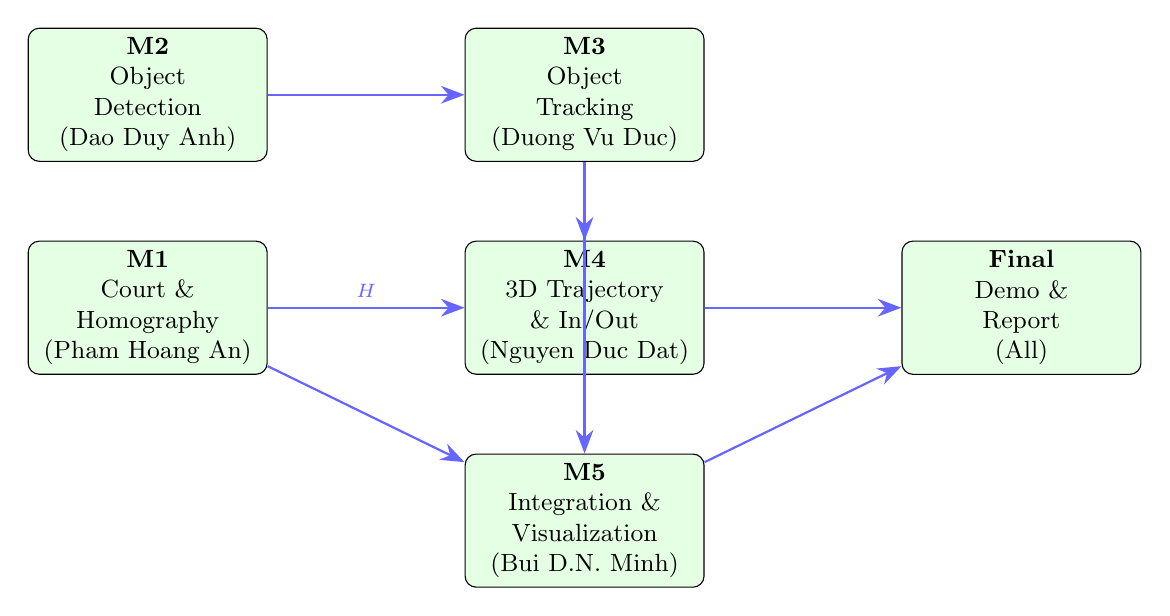
\begin{tikzpicture}[
  node distance=1.0cm and 2.5cm,
  mod/.style={rectangle, draw, fill=green!10, text width=2.8cm,
    align=center, rounded corners, minimum height=0.8cm, font=\small},
  arrow/.style={-{Stealth[length=3mm]}, thick, blue!60}
]
  \node[mod] (m1) {\textbf{M1}\\Court \&\\Homography\\(Pham Hoang An)};
  \node[mod, right=of m1] (m4) {\textbf{M4}\\3D Trajectory\\\& In/Out\\(Nguyen Duc Dat)};
  \node[mod, below=of m4] (m5) {\textbf{M5}\\Integration \&\\Visualization\\(Bui D.N. Minh)};
  \node[mod, above=of m1] (m2) {\textbf{M2}\\Object\\Detection\\(Dao Duy Anh)};
  \node[mod, right=of m2] (m3) {\textbf{M3}\\Object\\Tracking\\(Duong Vu Duc)};
  \node[mod, right=of m4] (final) {\textbf{Final}\\Demo \&\\Report\\(All)};

  \draw[arrow] (m1) -- node[above,font=\scriptsize]{$H$} (m4);
  \draw[arrow] (m1) -- (m5);
  \draw[arrow] (m2) -- (m3);
  \draw[arrow] (m3) -- (m5);
  \draw[arrow] (m4) -- (final);
  \draw[arrow] (m5) -- (final);
  \draw[arrow] (m3) -- (m4);
\end{tikzpicture}
\end{center}

\noindent
\textbf{Critical path:} M1 (Homography fix) $\rightarrow$ M4 (3D + In/Out)
$\rightarrow$ Final demo.  The homography fix is the \emph{highest
priority} because Modules 4 and 5 cannot produce correct court-mapped
results without a valid $H$.

\textbf{Parallel work:} M2 (Detection benchmarking) and M3 (Tracking
stabilisation) can proceed independently of M1.

% ============================================================================
\section{Milestones}
\begin{enumerate}
  \item \textbf{Milestone 1 -- Homography Fix (Pham Hoang An):}
        Robust corner selection, reprojection sanity check, temporal
        stabilisation.  Verified on multi-court test video.
  \item \textbf{Milestone 2 -- Detection Benchmark (Dao Duy Anh):}
        Comparative evaluation of all ball detection methods.  Optimised
        default configuration.  False-positive analysis.
  \item \textbf{Milestone 3 -- Stable Tracking (Duong Vu Duc):}
        DeepSORT integrated.  ID switch count minimised.  Ball trajectory
        smooth and continuous.
  \item \textbf{Milestone 4 -- Bounce/In-Out Validation (Nguyen Duc Dat):}
        Correct bounce detection on 3--5 validation clips.  In/out
        accuracy report.  Depends on Milestone~1.
  \item \textbf{Milestone 5 -- Final Demo (Bui Dinh Nguyen Minh + All):}
        Mini-map shows ball and players.  Court overlay on video.
        Final annotated output video.  Documentation and report
        submission.
\end{enumerate}

% ============================================================================
\section{Test Data and Validation}

\subsection{Primary Test Video}
\begin{itemize}[nosep]
  \item \textbf{File:} \texttt{data/raw/Video Project 4.mp4}
  \item \textbf{Resolution:} $1920 \times 1080$ pixels
  \item \textbf{Frame rate:} 30\,fps
  \item \textbf{Duration:} 1139 frames ($\approx$38 seconds)
  \item \textbf{Scene:} Outdoor tennis facility, camera positioned
        above/behind one baseline.  The main court is centre-left in
        the frame.  At least one adjacent court is visible on the right,
        which causes interference in court detection.
  \item \textbf{Match type:} Doubles (4 players on the main court).
\end{itemize}

\subsection{Latest Pipeline Results (Before Homography Fix)}
\begin{itemize}[nosep]
  \item Total frames processed: 1139
  \item Processing time: $\sim$636\,s (1.8\,fps on CPU)
  \item Ball detections: 633 / 1139 frames (55.6\%)
  \item Player detections: 4556 total ($\approx$4.0 per frame)
  \item Bounce events: 4 (all classified OUT --- likely incorrect due to
        bad homography)
  \item Output file: \texttt{outputs/Video\_Project\_4\_tracked.avi}
        (152\,MB)
\end{itemize}

\subsection{Validation Plan}
\begin{itemize}[nosep]
  \item Collect 3--5 additional clips covering: single court (clean lines),
        multiple courts, partial visibility, different camera angles.
  \item Manually annotate ball positions and bounce events on selected
        frames for quantitative evaluation.
  \item Report: detection rate, tracking continuity, homography
        reprojection error, bounce classification accuracy.
\end{itemize}

% ============================================================================
\section{Environment and Reproduction}

\subsection{Environment}
\begin{itemize}[nosep]
  \item OS: Windows 10/11
  \item Python 3.13, PyTorch 2.6+
  \item Key packages: \texttt{ultralytics} (YOLOv8), \texttt{opencv-python},
        \texttt{numpy}, \texttt{matplotlib}, \texttt{scipy}, \texttt{tqdm},
        \texttt{pyyaml}
  \item Optional: \texttt{deep-sort-realtime} (for DeepSORT tracker)
  \item Environment variable:
        \texttt{TORCH\_FORCE\_NO\_WEIGHTS\_ONLY\_LOAD=1}
\end{itemize}

\subsection{Installation}
\begin{lstlisting}[language=bash]
pip install ultralytics opencv-python numpy matplotlib scipy tqdm pyyaml
pip install deep-sort-realtime  # optional, for DeepSORT
\end{lstlisting}

\subsection{Running the Pipeline}
\begin{lstlisting}[language=bash]
cd tennis-pickleball-tracker
set TORCH_FORCE_NO_WEIGHTS_ONLY_LOAD=1
python run_pipeline.py
\end{lstlisting}

\subsection{Inspecting a Single Frame}
\begin{lstlisting}[language=bash]
python test_fix.py
# Output: outputs/test_results/annotated_frame_v2.jpg
\end{lstlisting}

% ============================================================================
\section{Conclusion}
The Tennis/Pickleball Single-Camera Tracking System successfully implements
an end-to-end pipeline from video input to annotated output.  Ball detection
achieves 55.6\% frame-level detection rate, player filtering correctly
identifies 4 on-court players per frame, and the tracking module produces
continuous trajectories.

The primary remaining challenge is the \textbf{incorrect homography} caused
by multi-court line interference (Section~\ref{sec:issue}).  This is the
highest-priority fix because it blocks correct 3D reconstruction, bounce
analysis, in/out classification, and mini-map rendering.  The proposed
fix (robust corner selection + reprojection sanity check + temporal
stabilisation) is well-defined and assigned to Pham Hoang An.

With the 5-member task allocation defined in Section~\ref{sec:tasks}, the
team is positioned to deliver a stable, evaluated system in the upcoming
milestones.

\end{document}
